%!TEX root = ../thesis.tex
%*******************************************************************************
%****************************** Second Chapter *********************************
%*******************************************************************************

\chapter{Medical Background}
\label{chapter1}

\ifpdf
    \graphicspath{{Chapter2/Figs/Raster/}{Chapter2/Figs/PDF/}{Chapter2/Figs/}}
\else
    \graphicspath{{Chapter2/Figs/Vector/}{Chapter2/Figs/}}
\fi

Measuring blood flow provides valuable information to the clinical community about the healthiness of either organs or limbs. Being capable of estimate instant blood flow of one of the limbs provide information about how blood flow is ultimately reaching these extremities that could avoid ischemia (\textit{isch} in Greek means to stop or block and \textit{emia} that means blood flow) or amputation caused by a non-proper perfusion to the extremity. In fact, if there were indicators about either venous or arterial occlusion could provide a clue about how to proceed with the proper treatment.

\mynote{This introduction needs to be improved. More about what I'm going to describe should be added}
The following chapter describes the importance of blood flow, the problems and complications derived from a poorly perfused limb could cause. During the continuation of the reading, some of the current technologies will be explained and what methods are used to estimate blood flow currently.  

\section{Blood and its components} %section 2.1
Blood is the main carrier of nutrients that runs through humans and vertebrate animals. It also takes a major part in the body's defence combating infections. In short, it is in charge of transporting oxygen and collecting carbon dioxide from all the tissues that constitute the body.  Blood requires of different paths to circulate in the human body; the circulatory system is used to carry oxygenated and deoxygenated blood, also known as arterial and venous blood respectively. Indeed, the body uses arteries to transport oxygenated blood coming out from the heart and uses veins to return deoxygenated blood to the heart.

\mynote{Add a description of which veins are involved in the periphery. And how works in the arm. Arm Anathomy}

%********************************** %Section 2.1.1  **************************************  
\subsection{Components of blood}
\label{section literature 1.1}
There are well known and identifiable components in blood. Approximately, half of its volume is constituted of plasma and the other half of red blood cells (erythrocytes), white blood cells (leukocytes or monocytes) and platelets (thrombocytes). Each of this cells has specific tasks and characteristics which as described in table \ref{table:cell} shows cells quantity in a microliter of human blood. It must be noted that there are diverse specialised subtypes of white cells and platelets but not further details of this cells will be covered in this work.

\begin{table}
\caption{Blood cell classification}
\label{table:cell}
\centering
\begin{tabular}{p{2.5cm} p{1.5cm} p{3.5cm} p{6.5cm}}
\toprule
\textbf{Cell Type }& \textbf{Quantity} & \textbf{Geometry} & \textbf{Characteristic} \\
\midrule
Red Blood Cells (RBCs ) \newline or erythrocytes & \numrange{5e6}{6e6} & Shape: Disk \newline Diameter: 6-\SI{8}{\micro\meter} \newline Thickness: \SI{2}{\micro\meter} & 
\begin{tabular}[t]{@{\textbullet~}p{6.5cm}@{}} 
    Principal medium to deliver oxygen \\
    Lack of nucleus \\
    Cytoplasm rich in negatively charged Iron–containing Hb \\
    Contains Ions of Sodium (Na+) and Potassium (K+) \\
    Typical bilayer lipid membrane (Lipid composition defies physical properties such as membrane permeability and fluidity) 
\end{tabular} \\
\midrule

White Blood Cells (WBC) \newline or Monocytes & \numrange{4e3}{11e3} & Shape: Irregular \newline Diameter: 10–\SI{20}{\micro\meter} \newline Monocytes: 14–17 & 
\begin{tabular}[t]{@{\textbullet~}p{6.5cm}@{}} 
    Composed five different type of specialised cells to target different illnesses\\
    Make part of the immune system \\
    High count of these cells are indicators of disease 
\end{tabular} \\
\midrule

Platelets & \numrange{150e3}{400e3} & Shape: Irregular \newline Diameter: 2–\SI{3}{\micro\meter}  &  
\begin{tabular}[t]{@{\textbullet~}p{6.5cm}@{}}
    Lack of nucleus  \\
    Responsible for procoauglant activity \\
    If count to low excessive blood may occur. Too high blood cloth might form (thrombosis)
\end{tabular} \\ 

\bottomrule
\end{tabular}
\end{table}

%********************************** %Section 2.1.2  **************************************
\subsection{Oxygen transportation}
\label{section literature 1.2}
Oxygen ($O_2$) is an essential component needed by all body's cells to complete metabolic processes. Within the blood, this is transported by haemoglobin (Hb) contained within red blood cells (RBCs). Oxygen is required for the chemical reactions needed to convert biochemical energy from nutrients coming from food into cell's energy known as coenzyme or adenosine triphosphate (ATP). As a result of this reaction waste product is released from the cell. A human cell can only survive for a few minutes without oxygen~\cite{culmsee2005apoptosis}.

Inadequate oxygen delivery to body's tissue is known as hypoxia. There are different classifications of hypoxia count based on its cause~\cite{marieb2007human} which are described as follows: 

\begin{enumerate}
    \item \textbf{Anaemic Hypoxia:} It is a condition where a body part or an organ has poor $O_2$ delivery. Some of the causes are a small count of RBCs and abnormal or too little Hb content in the blood's cells.
    \item \textbf{Ischemic (stagnant) hypoxia: }This is caused when blood circulation is reduced or blocked. There are different causes for this. However, the most commons are congestive heart failure that may cause body–wide hypoxia, emboli or thrombi blocking oxygen supply to the tissue distal from the occlusion. 
    \item \textbf{Histotoxic hypoxia: }Mainly caused by metabolic poisoning like ingestion of cyanide. In this case the cell is unable to use $O_2$ for metabolic purposes, even though there is an appropriate amount of $O_2$ being delivered by the body.
    \item \textbf{Hypoxemic hypoxia:} It is shown by a decrease in the arterial oxygen partial pressure ($PO_2$). Some of the causes are an imbalance in the ventilation–perfusion coupling mechanism, poor ventilation caused by pulmonary disease and breathing air with a low content of $O_2$. Moreover, carbon monoxide ($CO$) poisoning is another reason behind this illness because it has \num{200} times more affinity with Hb than $O_2$. Thus, in places with high concentration of CO such as fires could lead easily to death.
\end{enumerate}

%********************************** %Section 2.2  **************************************
\section{Problems derived from poor blood delivery} %Section 2.2
\label{section literature 2}
Now that has been described some of the problems of having a poor oxygen transportation of blood at a cellular level; more detail will be unveiled about illnesses due to the poor or total lack of blood delivery to human tissue especially human limbs. 

Ischemia develops when there is an insufficient supply of blood to an organ. For instance, if an artery blockage occurs all the tissue below the path will suffer from starvation of oxygen and other critical nutrients. Different causes could lead to the blockage of an artery which can be caused by external or internal factors. Speaking specifically of lower limbs, these represent a significant cause of disability and cardiovascular morbidity and mortality~\cite{novo1995patients}. 

Exists different kind of diseases compromising limbs, an example of this is peripheral arterial disease (PAD), which also originates in another kind of illnesses according to the kind of occlusion or blockage. For instance, critical limb ischemia (CLI), which is a condition where as a consequence of arterial disease, a patient experiments pain in the extremity even at rest or in a breakdown of the skin~\cite{novo2004critical}. 

Clinically there are different forms to assess the development of this illness. Some scales of qualitative evaluation have been developed such as the Rutherford classification, the Leriche-Fountaine classification or the TACS II classification of femoral and popliteal lesions~\cite{norgren2007inter}. Health practitioner uses a survey, an indicator of pain when walking and a visual inspection is possible to determine the stage or the severity of the arterial occlusion.  Table \ref{table:Fountaine}) shows the different stages of the Leriche-Fountain classification and the various steps considered to evaluate the illness.

\begin{table}
\caption{Leriche-Fountaine classification}
\centering
\label{table:Fountaine}
\begin{tabular}{p{1.8cm} p{3.8cm} p{3.5cm} p{4.5cm}}
\toprule
\textbf{Stages}& \textbf{Symptoms} & \textbf{Pathophysiology} & \textbf{Pathophysiological \newline classification} \\
\midrule
Stage I & Asymptomatic \newline or effort pain & Relative hypoxia & Silent Arteriopathy \\
\midrule
Stage II A & Effort pain \newline Pain free walking distance > \SI{200}{\meter} & Relative hypoxia & Stabilized Arteriopathy \newline Non-Invalidant claudication \\ 
\midrule
Stage III A & Rest Pain \newline Ankle arterial pressure > \SI{50}{\mmHg} & Cutaneous hypoxia \newline Tissue acidosis \newline Ischemic neuritis & Instable arteriopathy \newline Invalidant claudication \\
\midrule
Stage III B & Rest pain \newline Ankle arterial pressure < \SI{50}{\mmHg} & Cutaneous hypoxia \newline Tissue acidosis \newline Ischemic neuritis & Instable arteriopathy \newline
Invalidant claudication \\
\midrule
Stage IV & Trophic lesions \newline Necrosis or Gangrene & Cutaneous hypoxia \newline 
Tissue acidosis & Necrosis \newline Evolutive arteriopathy \\
\bottomrule
\end{tabular}
\end{table}

As table~\ref{table:Fountaine} shows, there are various levels of stratifying the severity of the disease according to the symptoms that are related pathophysiology. According to the gravity of the stage where the patient is, there are different methods to examine the severity of the disease using imaging methods. These will be described in detail in the section xxx.

\mynote{relate this to a section in the document later on}

There is another type of illness when the obstruction does not occur in an arterial vessel but around the microcirculation bed. An example of this is compartment syndrome. A cause of this disorder is the increase of pressure in a limb that leads to total or partial restriction of micro–vascular blood flow~\cite{songer2001tissue}. It commonly happens when proximal veins are occluded rather than deep vein thrombosis (DVT). Some cases also present rapid discoloration and blistering of the affected limb being commonly associated with oedema, cyanosis and severe pain~\cite{chhabra2013compartment} which can be classified using one of the methods described previously. In the end, ultimately could lead to venous hypertension and loss of blood plasma; as well as reduced arterial flow can result in gangrene, limb loss and possibly death~\cite{lamborn2014compartment}. Doppler sonography is one of the traditional techniques used to monitor this problem~\cite{chhabra2013compartment}. Nevertheless, detecting foot compartment syndrome could be challenging to detect compared to other parts of the body because its symptoms and indicators are less reliable~\cite{dodd2013foot}.  

The lack of blood towards an extremity can also be caused by a secondary effect of other illness like diabetes. Some of the most common problems that diabetic patients have to deal with are diabetic foot infection which is a clinical syndrome characterised by local findings of inflammation or purulence in a person with diabetes. Also, it also leads to a decrease in peripheral circulation, vascular disease and loss of nerve sensation ending up in the formation chronic ischemic ulcers and bacterial infection. Diabetes is the leading cause of lower extremity amputation in developed countries, and it is responsible for \SI{60}{\percent} of these amputations~\cite{ucckay2014diabetic}.  Currently, Doppler ultrasound flowmetry is still one of the primary tools to diagnose the advance of Diabetes foot infection (DFI). Although, new techniques to follow up the progress of this illness have been researched such as bioelectrical impedance~\cite{cheng2012application}, planar pressure analysis~\cite{dos2010insole}, imagine technique analysis~\cite{songer2001tissue}, near infrared~\cite{papazoglou2008assessment} and electronic noses~\cite{yusuf2013diagnosis}. Until now, nothing has been designed to detect early stages of this problem before ulceration occurs. Regarding bioelectrical impedance analysis (BIA), there have been studies focused on the detection on the development of ischemia of the foot's sole showing a good correlation with laser Doppler flowmetry~\cite{cheng2012application}. 

%********************************** %Section 2.2.1  **************************************
\subsection{Peripheral vascular disease}
\label{section literature 2.1}
Some of the common forms of reduction in blood towards a limb are known as the peripheral vascular disease (PVD) also known as peripheral arterial disease (PAD). This sickness is a progressive vascular condition caused by the blockage, narrowing, or spasms in a blood vessel (arteries, veins or lymphatic vessels). Hence, altering the blood circulation to and from any upper or lower extremities.  Most commonly affect the lower limbs, especially legs and feet. Therefore, the derivation of its name as "peripheral" because it affects mostly the periphery of the body. It affects \SI{5}{\percent} of people over \num{50} and between \SIrange{12}{20}{\percent} of people over 65 years old. To some extent, it is more common in men than women. People with certain risk factors are more likely to suffer PVD such as patients with diabetes of smokers.  

\mynote{I need a reference for this numbers}

Different factors could cause the narrowing of the blood vessels. The most common cause of PVD is atherosclerosis, deposition of fatty material on the arterial walls. This fatty material constitutes a plaque that reduces the blood flow towards tissue in the limb lessen the transport of $O_2$ and nutrients as explained in Oxygen transportation section. Moreover, clots may also form on the artery walls reducing the internal size of the vessel and increasing the risk of obstructing off a major artery. 

Different risk factors are contributing to the development of this sickness. Some can be inherited to the population others are based on lifestyle choices. The combination of two of more of the following risks may increase complications from PVD, such as smoking and diabetes. However, more in details some of the documented risk factors are:

\begin{itemize}[noitemsep]
    \item Age (especially over \num{50})
    \item Family history (high blood pressure, high cholesterol or PVD)
    \item Diabetes
    \item Smoking
    \item Obesity
    \item Infections
    \item Coronary artery disease
    \item Injury to vessels
    \item Physical inactivity
    \item High blood pressure
    \item Autoimmune diseases
    \item Nutritional deficiencies
    \item High blood cholesterol
    \item Emboli from other locations in the body
    \item Inflammation of the blood vessels
\end{itemize}

On the first stages of the illness, symptoms are not noticeable, which makes difficult to diagnose the condition. Just until it has been developed into a painful stage as described by the Fountaine's classification (see table \ref{table:Fountaine}) is when actions come into place. However, performing a qualitative assessment of the extremity helps to diagnose the sickness in early stages. Some of the indicators could be coldness to touch, poor skin condition (thinning, shining or brittle), poor nail health (thickening or opaque nails), hair loss in the extremity, reduced pulse sensation in the extremity, impotence, infections or injuries not healing properly, poor muscle condition (numbness, weakness or heaviness), pain while walking and stop at rest, local skin discolouration (pale, blue or dark red) and restricted mobility. 

Once a qualitative or physical examination has been performed, and the progress of the illness has been classified there are additional tests that may help to diagnose the severity of the PVD. Some of the methods just require the assessment of the medical practitioner using common medical devices others may need the use of specialised equipment. Some of the therapeutic methods that do not demand the use of bulky or cumbersome devices are:

\begin{itemize}
    \item \textbf{Ankle-branchial index (ABI):} It is the ratio of the differential measurement of systolic blood pressure measured at the ankle to that measured at the brachial artery [17]. For this it is required to compared the difference in blood pressure between the arm and the ankle, it also needed to record the ankle's blood flow using a Doppler ultrasound instrument.  
    \item \textbf{Treadmill exercise test: }In this method the patient has to walk or run to monitor the circulation during exercise. Pain or problems during the test are recorded to examine the severity of the obstruction.
    \item \textbf{Reactive hyperaemia test:} This test refers to a temporary increase (\textit{hyper}) of blood flow (\textit{emia}) of the extremity. It is usually performed in people who are not able to walk on a treadmill. In this case, the person is taken to supine position and comparative measurements of blood flow in tights and ankles are taken after occlusion to determine any decrease between both sites. 
\end{itemize}


\section{Plethysmography}
\label{section literature 3}
The word plethysmography roots from the Greek word \textit{plethymos} that means either increasing or enlarging and \textit{graphos} that is to write. In other words, it can be defined as the measurement of volume in the human body. In medicine, some of the common applications are the measurement of volume changes in lungs caused by the respiratory system or blood vessels caused by the circulatory system~\cite{turcott2004methods}.  More specifically when referring to the latter, plethysmography aims to measures the pulsatile volume changes when the heart pumps blood in and out in a segment of the human body. 


A plethysmography device produces an output waveform that is synchronous to the heart cycle. The shape of the signal is similar to an arterial pressure waveform. In fact, the plethysmography plot represents the volume of the arterial vasculature obtaining a measure of the arterial pulse amplitude. This waveform gives meaningful information about the pulse velocity and indications of possible arterial obstruction.

\begin{figure}[!htpb]
	\centering
	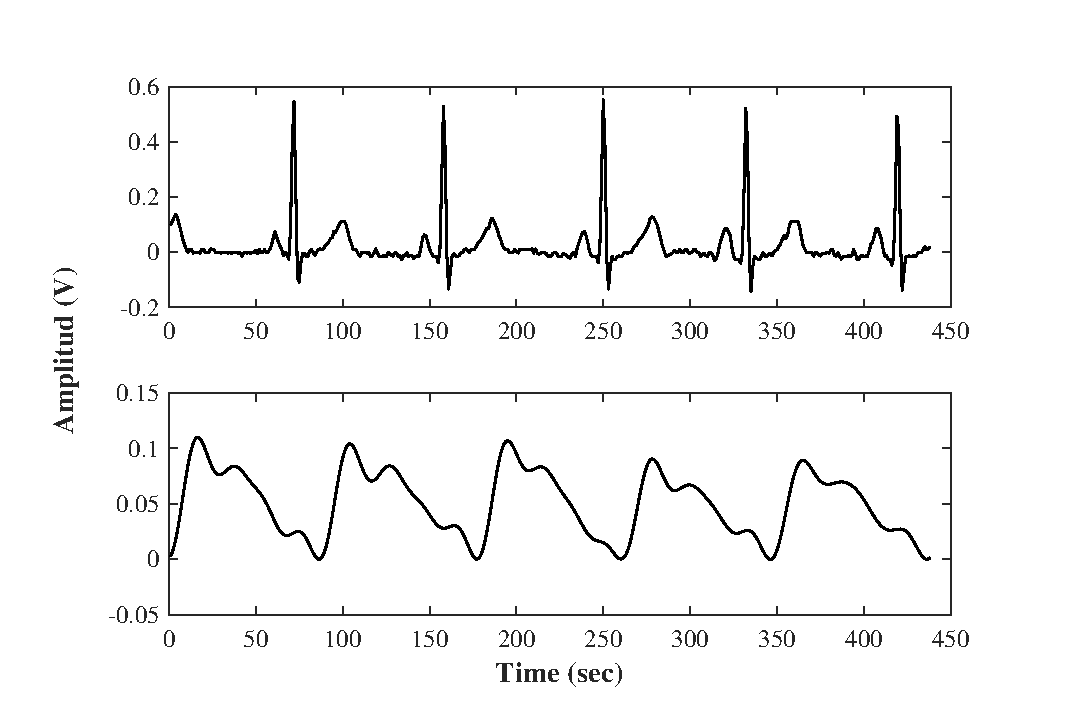
\includegraphics[width=0.75\textwidth,keepaspectratio]{figure1}    
	\caption[Classic plethysmography waveform]{Representation of a classic plethysmography waveform from the heart cycle. The image on the top represents the electrical signal of the heart (ECG). The one below is the plethysmography waveform of the circulation. Both signal are synchronous}
	\label{fig:plethysmography}
\end{figure}

There are different methods and technologies to measure plethysmography. Every method can be applied separately or as part of a system. Some techniques can measure plethysmography of the whole body, segments or localised areas. For instance, chambers of air or water are used to measure lung capacity. This chamber measures the air displacement of a patient while this inhales inside the chamber. 

For measurement of changes of volume of a limb's segment, the air plethysmography technique could be very cumbersome and not very practical. This is one of the many reasons why more techniques have been developed. The following section describes methods to detect plethysmography from a part of the body.

\subsection{Air plethysmography}
\label{section literature 3.1}
Air plethysmography is not a common method to measure a limb’s change of volume. It has been used as an either alternative or research method as explained by Chuah et al.~\cite{chuah2004plethysmography} for measurement of plethysmography without venous occlusion. This approach uses a special chamber that contains the limb in a close area with orifices where transducers and calibration devices are connected. The arm is introduced into the case through a tight rubber sleeve to ensure that the instrument is airtight.  The plethysmography pulsations are detected by measuring the displacement of the surrounding air with a sensor connected to the chamber, which also moves the rubber diaphragm which a Doppler ultrasound transducer measures displacement. As can be noticed, this method could be burdensome, and it is not very desirable to be applied during critical application such as surgery.

\begin{figure}[!htpb]
	\centering
	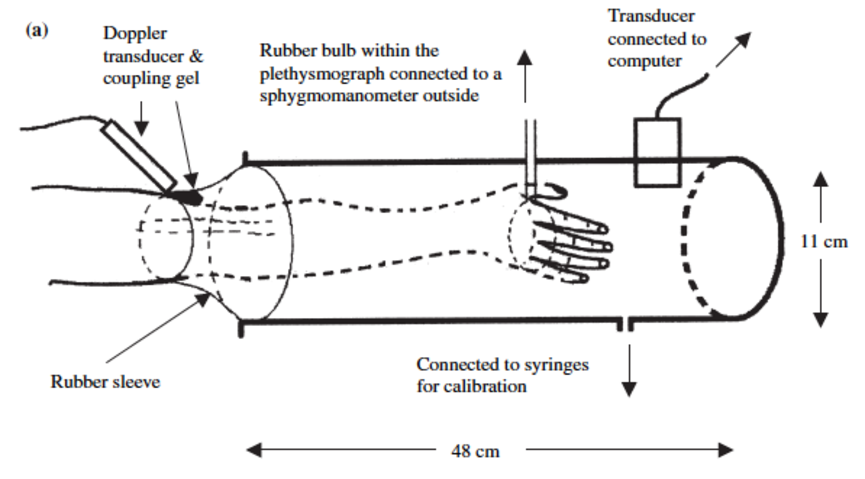
\includegraphics[width=0.95\textwidth,keepaspectratio]{figure_3_2}    
	\caption[Air plethysmography method]{Representation of an air plethysmography device. It requires a one side open cylinder with with a rubber sleeve. There is a compartment where the air displacement caused by each cardiac cycle can be measured.}
	\label{fig:air plethysmography}
\end{figure}

\subsection{Doppler method}
\label{section literature 3.2}
The Doppler technique is not directly a plethysmography method because it does not measure changes in volume but variations of flow. In physics, both parameters are related if the cross-section area of the volume being measured is known. Hence, if the flow and area are known is possible to deduce the volume flow rate. This method uses the Doppler effect to measure blood flow non-invasively from the skin surface. It is very popular in the medical ambit. It could be implemented via ultrasound (ultrasound Doppler flowmetry) frequency or photoelectric effect (laser Doppler flowmetry).  This method measures the velocity of particles in solution using frequency shift of backscattered ultrasound or light~\cite{orekhova2013doppler} (see Figure \ref{fig:Doppler method}). 

A signal is generated to a target tissue and then reflected by the macroscopic tissue structures. Some of the energy in light or sound form is reflected, absorbed and scattered by the tissue and blood particles. This method measures the microcirculation underlying the flow of the arterioles and venules. However, this technique is mainly for superficial measurements or invasively for free flap flow measurements. For instance, it has been studied that laser Doppler flowmetry has \SI{1}{\milli\meter} of penetration. In the case of ultrasound Doppler measurements are affected by the angle of the frequency applied to the target tissue.

\mynote{reference to this depth}

\begin{figure}[!htpb]
	\centering
	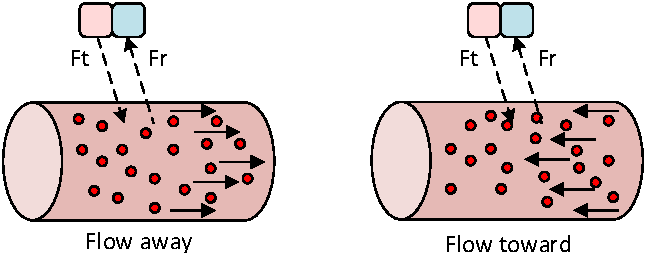
\includegraphics[width=0.75\textwidth,keepaspectratio]{figure_3_3}    
	\caption[Doppler technique to measure flow]{Representation of a classic plethysmography waveform from the heart cycle. The image on the top represents the electrical signal of the heart. The one before is the plethysmography waveform of the circulation.}
	\label{fig:Doppler method}
\end{figure}


\subsection{Strain gauge plethysmography}
\label{section literature 3.3}
This method also known as SGP (strain gauge plethysmography) is a non-invasive method to quantify retrograde outflow in the deep venous system and peripheral arterial disease~\cite{holohan1996plethysmography}. It works by applying a strain gauge around the limb under test. The transducer could be a tube filled in with a conductive material such as mercury and gallium and connected to a source of electricity. However, alternative methods that do not use clinically banned mercury have been developed using electrical conductive fluids~\cite{flowers1981strain}. When the gauge experiences variations of circumference caused by a change of volume of the rib cage or the pulse in a limb, the resistance of the sensor also vary accordingly obtaining an electrical waveform. To increase sensitivity for venous filling measurements occlusion cuffs would be required, as shown in Figure~\ref{fig:strain gauge}. This method does not provide reliable quantitative data for venous occlusion but provides qualitative data for the function of the extremity in venous insufficiency~\cite{holohan1996plethysmography}. 

\begin{figure}[!htpb]
	\centering
	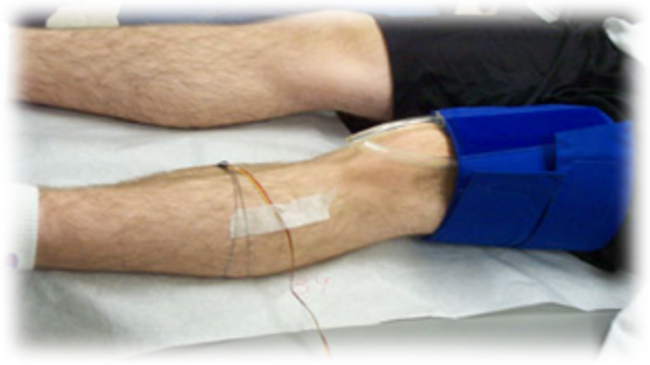
\includegraphics[width=0.75\textwidth,keepaspectratio,trim={0.5cm 0.5cm 0.5cm 0.5cm}, clip]{figure_3_4}    
	\caption[Strain gauge plethysmography]{Representation of a classic plethysmography waveform from the heart cycle. The image on the top represents the electrical signal of the heart. The one before is the plethysmography waveform of the circulation.}
	\label{fig:strain gauge}
\end{figure}


\subsection{Photoelectric method}
\label{section literature 3.4}
This method is technically known as photoelectric plethysmography or PPG for short. It is one of the most popular methods used in medical applications nowadays. It is a non-invasive method that uses different light wavelengths to obtain a plethysmography graph. It is widely used for monitoring or evaluating heart rate, oxygen saturation, peripheral arterial pressure and peripheral microcirculation after skin grafting, drug ingestion, burns or revascularization~\cite{holohan1996plethysmography}. There are two different techniques to obtain readings. One is transmission-mode (see Figure 2.20.a.) that works by placing the tissue of interest (i.e. finger, toe or ear lobe) between the light emitting diode (LED) and the receptor.  The other is PPG reflectance-mode (see Figure 2.20.b.) by placing the LED next to photoelectric cell over the surface of the tissue o study. PPG uses the AC component of the signal for arterial pulse detection and the DCcomponent for venous evaluation~\cite{higgins1986photoplethysmographic}. It also uses a different kind of wavelengths to avoid interference from external sources of light. The principle behind PPG is the detection of the degree of attenuation of backscatter light from the superficial layers of skin about \SIrange{1.5}{2.0}{\milli\meter} ~\cite{holohan1996plethysmography,kim1986pulse}. The amount of reflected light varies with the amount of RBC’s in the cutaneous microcirculation, which alters the wavelength during each cardiac cycle. This method has been proved to be effective for the initial diagnostics of peripheral arterial disease (PAD) and chronic peripheral venous insufficiency (CVI).

Some of the disadvantages of PPG are that only measures a small area at the time. Therefore, it is not possible to get a spatial distribution of the blood volume change over the skin~\cite{wu2003ppgi}. Also, skin pigmentation has been probed being an error factor as well as nail polishers~\cite{fallow2013influence}. 



Figure 2.20 – a) PPG transmission-mode b) PPG reflectance-mode

\subsection{Bioelectrical Impedance}
\label{section literature 3.5}
Also known as impedance plethysmography (iPG) involves the measurement of the change in impedance due to change of blood flow. For instance, when heart’s systole increases blood flow, the volume of a limb rises due to the inflow of blood (swelling)~\cite{martinsen2011bioimpedance}. Consequently, there are changes of impedance correlated to the changes of volume and flow in a limb. Some medical application might require the use of occlusion cuffs to analyse venous filling. There are several medical applications for this kind of technique such as heart stroke volume (SV) measurement, cardiac output (CO), thoracic respiratory volume, oedema and detection of deep vein thrombosis (DVT)~\cite{holohan1996plethysmography}.

The following section describes more in detail the definition of iPG, how it works, medical applications, how is measured and the possible ways to represent it. This information will help to understand how volume and ischemia can be related to calculating an index between the two measurements.

%********************************** %Nomenclatures in chapter  **************************************
\nomenclature[z-Hb]{Hb}{Haemoglobin}
\nomenclature[z-ATP]{ATP}{Adenosine Triphosphate}
\nomenclature[z-rbc]{RBC}{Red Blood Cells}
\nomenclature[z-abi]{ABI}{Ankle-Branchial index}
\nomenclature[z-wbc]{WBC}{White Blood Cells}
\nomenclature[z-PVD]{PVD}{Peripheral vascular disease}
\nomenclature[z-bia]{BIA}{Bioelectrical impedance analysis}
\nomenclature[z-DFI]{DFI}{Doppler flowmetry}
\nomenclature[z-DVT]{DVT}{Deep vein thrombosis}
\nomenclature[z-cli]{CLI}{Critical Limb Ischemia}
\nomenclature[z-PAD]{PAD}{Peripheral Arterial Disease}
\nomenclature[z-SV]{SV}{Strove Volume}
\nomenclature[z-LED]{LED}{Light emitting diode}
\nomenclature[z-CVI]{CVI}{Chronic peripheral venous insufficiency}
\nomenclature[z-ppg]{PPG}{Photoplethysmography}
\nomenclature[z-ipg]{iPG}{Impedance Plethysmography}
\nomenclature[z-CO]{CO}{Cardiac output}
\nomenclature[z-SGP]{SGP}{strain gauge plethysmography}
\nomenclature[z-BIA]{BIA}{Bioelectrical impedance analysis}


%\nomenclature[z-cif]{$CIF$}{Cauchy's Integral Formula}                                % first letter Z is for Acronyms 
%\nomenclature[a-F]{$F$}{complex function}                                                   % first letter A is for Roman symbols
%\nomenclature[g-p]{$\pi$}{ $\simeq 3.14\ldots$}                                             % first letter G is for Greek Symbols
%\nomenclature[g-i]{$\iota$}{unit imaginary number $\sqrt{-1}$}                      % first letter G is for Greek Symbols
%\nomenclature[g-g]{$\gamma$}{a simply closed curve on a complex plane}  % first letter G is for Greek Symbols
%\nomenclature[x-i]{$\oint_\gamma$}{integration around a curve $\gamma$} % first letter X is for Other Symbols
%\nomenclature[r-j]{$j$}{superscript index}                                                       % first letter R is for superscripts
%\nomenclature[s-0]{$0$}{subscript index}                                                        % first letter S is for subscriptsd
